\documentclass[12pt, a4paper]{article}
\usepackage[utf8]{inputenc}
\usepackage{listings}
\usepackage{courier}
\usepackage{fancyhdr}
\usepackage{color}
\usepackage{xcolor}
\usepackage{caption}
\usepackage{graphicx}
\usepackage{url}
\usepackage[titletoc]{appendix}
\usepackage{textcomp}
\usepackage{pdfpages}
\usepackage[colorlinks]{hyperref}
\usepackage{amsmath}
\usepackage{amssymb}
\usepackage{booktabs}
\usepackage{graphicx}
\usepackage{xcolor}
\hypersetup{
    colorlinks,
    linkcolor={black},
    urlcolor={blue}
}
\usepackage{tabularx,ragged2e}

\usepackage[british,english]{babel}
\usepackage{biblatex}
\addbibresource{bibliography.bib}
\DeclareFieldFormat{url}{Available at: \url{#1}}



\definecolor{light-gray}{gray}{0.95}

\lstset{
 upquote=true,
 showspaces=false,
 showtabs=false,
 frame=none,
 tabsize=2,
 breaklines=true,
 numbers=none,
 showstringspaces=false,
 breakatwhitespace=true,
 escapeinside={(*@}{@*)},
 keywordstyle=\bfseries,
 basicstyle=\footnotesize\ttfamily,
}

\newcommand{\code}[1]{{\footnotesize\texttt{#1}}}

\setlength\parindent{0pt} % Indentazione paragrafi
\setlength{\parskip}{1ex plus 0.5ex minus 0.2ex} % Spaziatura paragrafi

\renewcommand{\labelenumii}{\theenumii}
\renewcommand{\theenumii}{\theenumi.\arabic{enumii}.}

\pagestyle{fancy}
%\renewcommand{\chaptermark}[1]{\markboth{#1}{}}
\renewcommand{\sectionmark}[1]{\markright{\thesection\ #1}}
\fancyhf{}
\fancyhead[LE,RO]{\bfseries}
\fancyhead[LO]{\bfseries\rightmark}
\fancyhead[RE]{\bfseries\leftmark}
\renewcommand{\headrulewidth}{0.5pt}
\renewcommand{\footrulewidth}{0pt}
\addtolength{\headheight}{0.5pt}
\fancypagestyle{plain}{%
	\fancyhead{}
	\renewcommand{\headrulewidth}{0pt}
}
\rfoot{Page \thepage}


\title{Blockchain and cryptocurrencies}
\date{}
\author{Michele Zanotti}

\begin{document}

  \maketitle
  \tableofcontents

  \begin{enumerate}
    \item Preliminary concepts at the basis of Blockchain \cite{bambara2018blockchain},\cite{bashir2017mastering}
    \begin{enumerate}
      \item Introduction to the cryptography concepts used in Blockchain \cite{bashir2017mastering}
      \begin{itemize}
        \item Cryptography services (confidentiality, authentication, integrity, non-repudiation)
        \item Public and private key cryptography
        \item Elliptic curve cryptography
        \item Hash functions
        \item Elliptic curve digital signature algorithm (ECDSA)
      \end{itemize}
      \item Distributed systems and decentralization
      \item Consensus \& Byzantine generals problem
    \end{enumerate}

    \item Introduction to Blockchain \cite{bambara2018blockchain},\cite{bashir2017mastering}
    \begin{enumerate}
      \item What is a Blockchain
      \item Blockchain features
      \item Types of Blockchain (public, consortium, private)
      \item Blockchain history (why it was invented)
      \item Overview of today Blockchain applications
    \end{enumerate}

    \item Bitcoin \cite{karame2016bitcoin},\cite{antonopoulos2017mastering}
    \begin{enumerate}
      \item Bitcoin protocol specification
      \begin{itemize}
        \item Overview of Bitcoin data types (transaction, scripts, adresses, blocks)
        \item Transactions
        \item Bitcoin network architecture
        \item Bitcoin blockchain (blocks structure, Merkle trees, mining, proof of
        work)
      \end{itemize}
      \item Bitcoin wallets
%      \item Security of Bitcoin transactions
    \end{enumerate}

    \item Bitcoin privacy
    \begin{itemize}
      \item Considerations on user anonymity in Bitcoin
      \item Possible attacks
      \item How to enhance privacy in Bitcoin (explanation of mixing services
      + reference \cite{heilman-blindly-signed-contracts},\cite{saxena-bitcoin-anonymity})
    \end{itemize}

    \item Bitcoin blockchain scalability
    \begin{itemize}
      \item Considerations on the scalability of the Bitcoin blockchain and
      possibile solutions \cite{karame2016bitcoin},\cite{croman-scaling-blockchain}
    \end{itemize}

    \item Alternatives to Bitcoin
    \begin{itemize}
      \item Bitcoin limitations
      \item Alternatives to proof of work \cite{bentov-no-proof-of-work}
      \item Namecoin
      \item Litecoin
      \item ZCash
    \end{itemize}

%    {
%    \color{gray}

%    \item Smart contracts
%    \begin{itemize}
%      \item History
%      \item What smart contracts are
%      \item Security
%    \end{itemize}

%    \item Ethereum
%    \begin{itemize}
%      \item History
%      \item Ethereum components (Keys, addresses, accounts)
%      \item Ethereum blockchain
%      \item Ethereum network
%      \item Ethereum transactions
%      \item Ethereum virtual machine
%    \end{itemize}


%    \item (Possibly) Pratical example of blockchain application:
%    development of a distributed application through Ethereum Solidity
%    (Something similar to the application development shown in reference \cite{bambara2018blockchain})
%    }
  \end{enumerate}

  \section{Introductory concepts}

%%%%%%%%%%%%%%%%%%%%%%%%%%%
% *** FIRST SUB-SECTION ***
%%%%%%%%%%%%%%%%%%%%%%%%%%%
\subsection{Hash functions}
A hash function is a fuction that maps an arbitrary long input string to a fixed
length output string. Let $h$ refer to an hash function of length $n$:

\[
  h\colon \{0,1\}^* \to \{0,1\}^n
\]

$m$ is usually called ``the message'', while $d$ is usually called ``the digest``
and it can be seen as a compact representation of m. The length of $d$ is the

Hash functions are usually used to provide data integrity and they're also used to
construct other cryptographic primitives such as MACs and digital signatures.

\subsubsection{Desired properties}
An hash function should ideally meet these properties:
\begin{itemize}
  \item \textbf{Computational efficiency}: given m, it must be easy to compute ${d=h(m)}$
  \item \textbf{Preimage resistance} (also called \textbf{one-way property}):
  given ${d=h(m)}$, it must be computationally infeasible computing $m$ ($m$ is the
  preimage)
  \item \textbf{Weak collision resistance} (also called
  \textbf{2\textsuperscript{nd} preimage resistance}): given $m_1$ and ${d_1=h(m_1)}$,
  it must be computationally infeasible finding a $m_2 \neq m_1$ so that ${h(m_2)=d_1}$
  \item \textbf{Strong collision resistance}: it must be computationally infeasible
  finding pairs of distinct and colliding messages. Two messages $m_1\neq m_2$
  collide when ${h(m_1)=h(m_2)}$.
  \item \textbf{Avalanche effect}: changing a single bit of $m$ should cause every
  bit of ${d=h(m)}$ to change with probability ${P=0.5}$
\end{itemize}

\subsubsection{Examples of hash functions}
\begin{itemize}
  \item \textbf{MD5}: published in 1991, it's a 128-bit hash function that was
  used for file integrity checks. Today it's considered insecure and it shouldn't
  be used anymore.
  \item \textbf{Secure Hash algorithm 1 (SHA-1)}: 160-bit hash function that was
  used in SSL and TLS implementations. Today is considered insecure and it's
  deprecated.
  \item \textbf{SHA-2}: family of SHA functions which includes SHA-256, SHA-384
  and SHA-512. SHA-256 is currently used in several parts of the Bitcoin network.
  \item \textbf{SHA-3}: latest family of SHA functions, it is a NIST-standardized
  version of Keccak, which uses a new approach called ``sponge construction''
  instead of the Merkle-Damgard transformation previously used. This family
  includes SHA3-256, SHA3-384 and SHA3-512.
\end{itemize}












\subsubsection{Design of SHA-256} SHA-256 works on 512-bits blocks and the input
message size has to be $< 2^{64}$bit. The outpus size is 256 bits. The algorithm
can be divided in two phases: pre-processing and hash computation.

\paragraph{Pre-processing}
\begin{enumerate}
  \item Padding of the message so that its length is a multiple of 512 bits.
  \item Parsing the message into N blocks of 512 bits $M(0), M(1), \dots, M(N)$.
  The first 32 bits of a block $i$ are denoted $M_0(i)$, the next 32 bits
  are $M_1(i)$ and so on up to $M_{15}(i)$.
  \item Setup of the initial has value $H(0)$, which is a sequence of eight 32-bits
  words obtained by taking the first 32-bits of the fractional parts of the
  square roots of the first eight prime numbers.
\end{enumerate}


\paragraph{Hash computation} The blocks of the message are processed one at a
time, beginning with $H(0)$, as follows:
\[ H(i) = H(i-1) + C_{M(i)}(H(i-1)) \]
where $+$ is the $\bmod 32$ addition and $C$ is the SHA-256 compression function,
which is shown if figure \ref{fig:sha256-compress-function} and it's basically
a block cipher which uses the message block $M(i)$ as key.

$H(N)$ is the hash of the message $M$.

\begin{figure}[!htb]
	\centering
	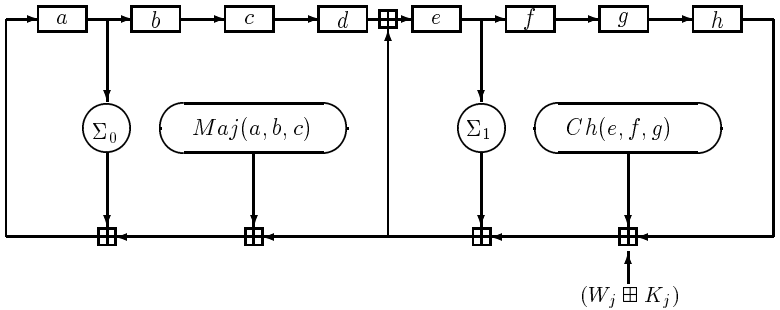
\includegraphics[width=1\linewidth]{img/sha-256-round.png}
	\caption{A round of the SHA-256 compress function $C$. The symbol $\boxplus$
  denotes the $\bmod 32$ addition, $Maj(X, Y, Z)=(X \cap Y) \oplus (X \cap Z) \oplus (Y \cap Z)$,
  $Ch(X,Y,Z)=	(X \cap Y) \oplus (!X \cap Z)$, $W_j$ and $K_j$ and round constants
  and $\sum_0$ and $\sum_1$ perform bitwise rotation.}
	\label{fig:sha256-compress-function}
\end{figure}

















\subsubsection{Message Authentication Codes (MACs)}
A MAC is an hash function which uses a key and which can therefore be used to
provide both integrity and authentication (proof of origin). Authentication is
based on a key pre-shared between the sender and the receiver. The receiver can
verify both integrity and authentication of a message by computing the MAC function
of the message and comparing it with the one received from the sender: if they are the
same then integrity and authentication are confirmed (note that it is assumed that
only the sender and the receiver know the key).

MAC functions can be constructed using block ciphers or hash functions:
\begin{itemize}
  \item in the first approach, block ciphers are used in the Cipher block chaining mode (CBC mode):
  the MAC of a message will be the output of the last round of the CBC operation.
  The length of MAC, in this case, is the same as the block length of the block cipher
  used to generate it.
  \item In the second approach, they key is hashed with the message using a certain
  construction scheme. The most simple ones are \emph{suffix-only} and
  \emph{prefix-only}, which however are weak and vulnerable:
  \begin{itemize}
    \item suffix-only: ${d=MAC_k(m)=h(m|k)}$, where $h$ is an hash function
    \item prefix-only: ${d=MAC_k(m)=h(k|m)}$, where $h$ is an hash function
  \end{itemize}
\end{itemize}





\subsection{Digital signature}
Digital signatures are used to associate a message with the entity from which the
message has been originated. They provide the same service as MACs (authentication
and non-repudiation) plus the non-repudiation.

Digital signature is based on public key cryptography: Alice can sign a message
by encrypting it using its private key. Usually, however, for efficiency and security
reasons, Alice doesn't encrypt the message but its digest (hash of the message).
Figure \ref{fig:digital-signature} shows how a generical digital signature function
works.

An example of digital signature algorithms are RSA and ECDSA.

\begin{figure}[!htb]
	\centering
	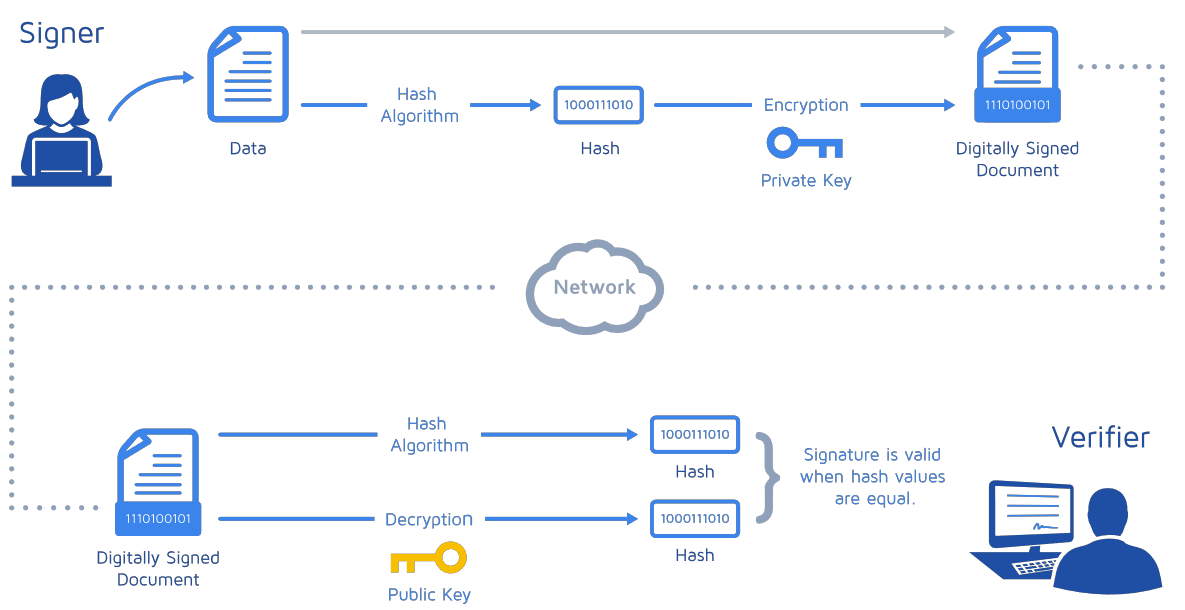
\includegraphics[width=1\linewidth]{img/digital-signature.png}
	\caption{digital signature signing and verification scheme}
	\label{fig:digital-signature}
\end{figure}





\subsection{Elliptic Curve Digital Signature Algorithm (ECDSA)}
ECDSA is a variant of the Digital Signature Algorithm (DSA) which uses elliptic
curve cryptography.

\subsubsection{Key pair generation}
\begin{enumerate}
  \item Define an elliptic curve $E$ with modulus $P$, coefficients $a$ and $b$ and a
  generator point $A$ that forms a cyclic group of order $p$, with $p$ prime
  \item Choose a random integer $d$ so that ${0 < d < q}$
  \item Compute the public key $B$ so that ${B = d  A}$
\end{enumerate}
The public key is the sextuple ${K_{pb} = (p,a,b,q,A,B)}$, while the private key
is the value of $d$ randomly chosen in Step 2: ${K_{pr} = d}$

\subsubsection{Signing a message}
\begin{enumerate}
  \item Choose an ephemeral key $K_e$, where ${0 < K_e < q}$.
  It should be ensured that $K_e$ is truly random and no two signatures have the same key
  because otherwise the private key can be calculated
  \item Compute ${R = K_e A}$
  \item Initialize a variable $r$ with the x coordinate value of the point $R$
  \item The signature on the message $m$ can be calculated as follow:
  \[{S=(h(m)+d r)K_e^{-1}\bmod q}\]
  where $h(m)$ is the hash of the message $m$. The signature is the pair ${(S,r)}$.
\end{enumerate}

\subsubsection{Signature verification}
A signature can be verified as follow:
\begin{enumerate}
  \item Compute ${w=S^{-1}\bmod q}$
  \item Compute ${u_1=w  h(m)\bmod q}$
  \item Compute ${u_2=w  r \bmod q}$
  \item Calculate the point ${P=u_1  A + u_2  B}$
  \item The signature ${(S,r)}$ is accepted as a valid signature only if:
   \[{X_P=r \bmod q}\]
   where $X_P$ is the x-coordinate of the point P calculated in Step 4
\end{enumerate}








%%%%%%%%%%%%%%%%%%%%%%%%%%%
% *** SECOND SUB-SECTION ***
%%%%%%%%%%%%%%%%%%%%%%%%%%%
\subsection{Blind signature} Blind signatures were introduced by David Chaum in
1982 \cite{chaum1982blind} and refer to a cryptographic primitive that allows an
entity to digitally sign a message without knowing or being able to read the
message that it signs. The following analogy introduced by Chaum himself clearly
explains what blind signatures are:

``\emph{Assume an envelope with both a piece of paper (e.g. a contract) and carbon
paper inside it. The envelope is sealed and sent to the signer. The signer
cannot see what is inside the envelope without breaking the seal. The signer
signs the envelope, and thanks to the carbon paper, the contract inside the
envelope gets signed too. The signer returns the envelope to the sender, who
opens it and extracts the carbon-signed contract.}''

Blind signature can be implemented using different schemes. In this section it will be
briefly discussed the RSA scheme proposed by Chaum. Another scheme based on the
Diffie-Hellman problem will be discussed in section \ref{sec:enh-sign}.

\subsubsection{RSA signature scheme} In RSA the public parameters are $n=pq$ and
a chosen $e$ relatively prime to $\varphi(n)$, while the private parameters are
the primes $p,q$, $\varphi(n)$ and \mbox{$d=e^{-1}\bmod\varphi(n)$}. The signer private
key is $d$ and its public key is $e$.

The signer can sign a message $m$ by computing the signature $s$:
\[ s=m^d\bmod n \]
Anyone can verify the signature using the signer public key and verify if the message
is equal to the result of the computation below:
\[ s^e = m^{ed}\bmod n= m \bmod n \]

\subsubsection{RSA blind signature scheme}
\begin{enumerate}
  \item Generation of a blinding factor $b=r^{e}\bmod n$,
  with $r$ random number
  \item The message $m$ is blinded with the blinding factor $b$ previously
  calculated: $m_{*}=b\cdot m\bmod n$
  \item The blinded message $m_*$ is sent to the signer. The signer signs it by
  computing $s_*$:
  \[ s_*=m_*^d\bmod n = b^d\cdot m^d\bmod n = r^{e\cdot d}\cdot m^d \bmod n = r\cdot m^d \bmod n \]
  \item The user can divide $s_*$ by $r$ for retrieving $s=m^d\bmod n$, namely
  the RSA signature of the message $m$
\end{enumerate}











%%%%%%%%%%%%%%%%%%%%%%%%%%%
% *** THIRD SUB-SECTION ***
%%%%%%%%%%%%%%%%%%%%%%%%%%%
\subsection{Distributed systems}
\subsubsection{What is a distributed system}
Blockchain at its core is basically a distributed system, therefore it is essential
to understand distributed systems before understanding Blockchain.

A distributed system is a network that consists of autonomous nodes, connected
using a distribution middleware, which acts in a coordinated way (passing
messages to each other) in order to achieve a common outcome and that can be
seen by the user as a single logical platform.

A node is basically a computer that can be seen as an individual player inside
the distributed system and it can be honest, faulty or malicious. Nodes that
have an arbitrary behavior (which can be malicious) are called \emph{Byzantine nodes}.

\begin{figure}[!htb]
	\centering
	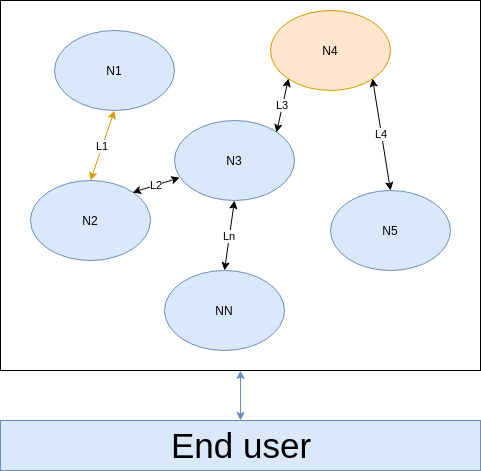
\includegraphics[width=0.6\linewidth]{img/distributed-system.png}
	\caption{design of a distributed system. N4 is a Byzantine node while L1 is a
  broken/slow network link}
	\label{fig:distributed-system}
\end{figure}

The main challenge in a distributed system is the fault tolerance: even if some
of the nodes fault or links break, the system should tolerate this and should
continue to work correctly. There are essentially two types of fault: a simple node
crash or the exhibition of malicious or inconsistent behavior arbitrarily. The
second case is the most difficult to deal with and it's called \emph{Byzantine
fault}. In order to achieve fault tolerance, replication is usually used.

Desired properties of a distributed system are the following:
\begin{itemize}
  \item \textbf{Consistency}: all the nodes have the same lates available copy of
  the data. It is usually achieved through consensus algorithms which ensure that
  all nodes have the same copy of the data
  \item \textbf{Availability}: the system is always working and responding to the
  input requests without any failures
  \item \textbf{Partition tolerance}: if a group of nodes fails the distributed
  system still continues to operate correctly
\end{itemize}
There is however a theorem, the \emph{CAP theorem}, which states (and proves)
that a distributed system cannot have all these three properties at the same time.
In particular, the theorem states that in the presence of a network partition (due
for example to a link failure) one has to choose between consistency and availability.



\subsubsection{Consensus}
Consensus is the process of agreement between untrusted nodes on a data value.
When the involved nodes are only two it's really easy to achieve consensus, while
in a distributed system with more than two nodes it is really hard (in this case
the process of achieving consensus is called \emph{distributed consensus}).
The data value agreed is the majority value, therefore the value proposed by
51\% of the nodes.

A consensus mechanism must meet these requirements:
\begin{itemize}
  \item \textbf{Agreement}: all the correct (non-faulty/malicious) nodes must agree on the same value
  \item \textbf{Termination}: the execution of the consensus process must come
  to an end and the nodes have to reach a decision
  \item \textbf{Validity}: the agreed value must have been proposed by at least
  one honest node
  \item \textbf{Fault tolerance}: the consensus algorithm must be able to run even
  in the presence of one or more Byzantine (faulty or malicious) nodes
  \item \textbf{Integrity}: the nodes make decisions only once in a single
  consensus cycle (in a single cycle a node cannot make the decision more than once).
\end{itemize}




\subsubsection{The Byzantine Generals Problem (BGP)}
The Byzantine Generals Problem (BGP) is a problem described by Leslie Lamport
\cite{lamport1982byzantine} in which a group of generals are surrounding a city
and they have to formulate a plan for attacking it (simplifying, they have to
decide whether to attack or retreat from the city).
Their only communication way is the messenger and they have to
agree on a common decision. The issue is that some of the generals may be
traitors trying to prevent the loyal generals from reaching an agreement by
communicating a misleading message. The generals need an algorithm to guarantee
that all the loyal generals agree on the same plan (attack or retreat) regardless
of what traitors generals do. Loyal generals will always do what the algorithm says they
should, while the traitors may do anything they wish.

As an analogy with distributed systems:
\begin{itemize}
  \item generals can be considered as nodes
  \item traitors can be considered Byzantine nodes
  \item the messenger can be seen as the channels of communication between the generals.
\end{itemize}

The problem can be see in term of generals-lieutenants: a General makes the
decision to attack or retreat, and must communicate the decision to his lieutenants.
Both the lieutenants and the general can be traitors: they cannot be relied upon
to properly communicate orders (traitor generals) and they may actively alter
messages in an attempt to subvert the process (traitor lieutenants).
\begin{figure}[!htb]
	\centering
	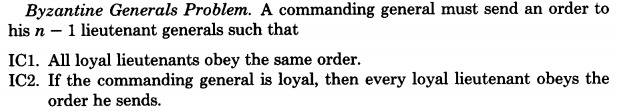
\includegraphics[width=1\linewidth]{img/byzantine-generals-problem.png}
	\caption{page 3 of the original Lamport's paper \cite{lamport1982byzantine}}
	\label{fig:byzantine-generals-problem}
\end{figure}

To solve this problem, Lamport proposed an algorithm for reaching consensus that
assumes that there are $m$ traitors and $3m$ actors. This implies that the
algorithm can reach consensus only if $2/3$ of the actors are honest: if the
traitors are more than $1/3$, consensus cannot be reached. The goal is
to make the majority of the lieutenants choose the same decision (not a specific one).
The original algorithm proposed by Lamport is shown in figure \ref{fig:lamport-byzantine-algorithm}.
\begin{figure}[!htb]
	\centering
	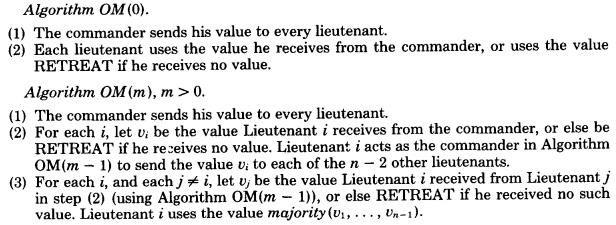
\includegraphics[width=1\linewidth]{img/lamport-byzantine-algorithm.png}
	\caption{Lamport's algorithm for reaching consensus}
	\label{fig:lamport-byzantine-algorithm}
\end{figure}



\subsubsection{Byzantine Fault Tolerance (BFT)}
A distributed system is said to be Byzantine Fault Tolerant when it tolerates a
the class of failures that belong to the Byzantine Generals’ Problem \cite{byzantine-konstantopoulos}.
In other words, a Byzantine Failure is a fault that presents different symptoms
to different observers and for this reason BFT is really difficult to achieve.

For example, a Byzantine Fault could be a node acting as a ``traitors'' and
generating arbitrary data during the process of reaching consensus.

  \section{Introduction to Blockchain}
\subsection{What is Blockchain}
From a technical point of view, Blockchain is a distributed ledger that is cryptographically
secure, append-only, immutable (extremely hard to change), and updateable only
via consensus among nodes.

From a business point of view, a blockchain can be defined as a platform
whereby peers can exchange values without the need for a central trusted party
by using transactions which are stored inside the blockchain in a verifiable and
permanent way.












\subsection{Blockchain features}

\subsubsection*{Decentralization}
This is the core feature of Blockchain. Thanks to decentralization there's no
need of a central trusted entity which stores the data and validates the
transaction, since the same copy of the Blockchain is stored by every node and
the validation of transaction is achieved through consensus.

\subsubsection*{Distributed consensus}
Blockchain has a high Byzantine Fault Tolerance\footnote{without BFT, a peer
would able to transmit and post false transactions} and allows to achieve
distributed consensus, therefore allows to have a single version of a data value
agreed by all parties without requiring a central authority.

\subsubsection*{High availability}
Blockchain is based on a peer-to-peer network of thousands of nodes and data is
replicated on each node, therefore the whole system is highly available since even
if one or more nodes fail the whole network can continue to work correctly.


\subsubsection*{Immutability}
All the data stored in a blockchain is immutable: once a block has been added to
the blockchain, it is considered practically impossible to change it (changing it
is computationally infeasible since it would require an unaffordable amount of
computing resources).

\subsubsection*{Transparency}
Blockchain is shared between the nodes and everyone can see what is in the
blockchain, thus allowing the system to be transparent and trusted.

\subsubsection*{Security}
Blockchain ensures the integrity and the availability of the data. Since
private keys and digital signatures are used, it also provide authentication and
non-repudiation. It doesn't provide confidentiality, due to it's transparency
feature (privacy is however required in certain scenarios, thus research in
this area is being carried out).

Blockchain security is due especially to its distributed nature, since for an
attacker would be a lot easier to tamper with data if it was stored on a single
central entity.

\subsubsection*{Uniqueness}
In Blockchain every transaction is unique and has not been spent already.
This is especially useful in cryptocurrencies applications of Blockchain,
where avoidance of double spending is a key requirement.















\subsection{Blockchain structure}
As shown in figure \ref{fig:blockchain-basic-schema}, a blockchain consists of a
linked list of ordered fixed-length blocks, each of which includes a set of transactions.
In this section, the generic elements of a blockchain will be presented.
\begin{figure}[!htb]
	\centering
	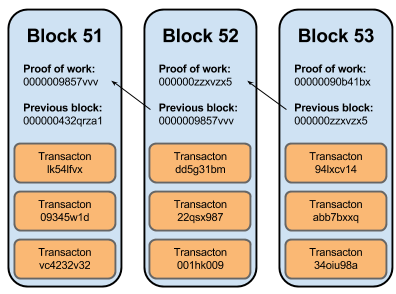
\includegraphics[width=0.5\linewidth]{img/blockchain-basic-schema.png}
	\caption{basic blockchain schema}
	\label{fig:blockchain-basic-schema}
\end{figure}

\subsubsection*{Blocks}
A block groups transactions in order to organize them logically and its size
depends on the blockchain implementation. Generally, a block is composed of:
\begin{itemize}
  \item a set of transactions
  \item a hash which identifies the block
  \item a pointer to the previous block hash (unless it's the genesis block)
  \item a nonce
  \item a timestamp
\end{itemize}
The \emph{genesis block} it's simply the first block in the blockchain and therefore
it can't contain any reference to the previous block.


\subsubsection*{Addresses}
Addresses are unique identifiers which identify the parties involved in a
transaction. An address is usually a public key or it's derived from a public key.


\subsubsection*{Transactions}
A transaction is a transfer of value from an address to another.


\subsubsection*{Peer-to-peer network}


\subsubsection*{Transaction scripts}
Transaction scripts are predefined sets of commands for nodes to transfer values
from one address to another and perform various other functions.


\subsubsection*{Programming language and Virtual machine} A Turing-complete
programming language is an extension of transaction scripts and it allows the
peers to define the operations that have to be performed on a transaction,
without the limitations of a non-Turing-complete transaction script. Programs
encapsulate the business logic and can, for example, transfer a value from one
address to another only if some conditions are met.

A virtual machine allows Turing-complete code to be run on a Blockchain as
smart contract (e.g. Ethereum virtual machine).

Not every Blockchain supports Turing-complete programming languages and virtual
machines (e.g. Bitcoin is not Turing-complete\footnote{It however supports
smart contracts}).


\subsubsection*{Nodes}
A node is an active entity which stores a copy of the blockchain and can perform
and/or validate transactions (following a consensus protocol, e.g. the Proof of Work).









\subsection{Consensus in Blockchain} Consensus in Blockchain is required to
establish whether the ledger itself or a piece of information submitted to it
are valid or not. In analogy with the Byzantine Generals Problem, the
``generals/lieutenants'' are the nodes participating in the blockchain, the
messengers are the network used by the nodes for communicating and the
``traitors'' are the nodes which try to tamper with the data by submitting, for
example, false data or by modifying the existing blocks.

In today Blockchain implementations are used four main consensus mechanisms:
the Practical Byzantine Fault Tolerance (PBFT), the Proof of Work (PoW),
the Proof of Stake (PoS) and the Delegated Proof of Stake (DPoS).

\subsubsection{Practical Byzantine Fault Tolerance Algorithm (PBFT)} The PBFT is
an algorithm proposed by M. Castro and B. Liskov as an optimized solution to the
Byzantine Generals Problem (more in general, it is an efficient replication
algorithm that is able to tolerate Byzantine faults \cite{castro1999practical}).

Simplifying, the algorithm works as follows \cite{blockchain-consensus-medium},
\cite{castro1999practical}: each ``general'' maintains an internal state and
when he receives a message, he uses the message in conjunction with his internal
state to run a computation, which tells to the general what to think about the
message in question. After reaching his individual decision about the message,
the general shares that decision with all the other ``generals'' in the system.
A consensus decision is determined based on the total decisions submitted by all
generals.


The advantage of this method is that is very efficient and allows to establish
consensus with less effort than other methods. The main disadvantage is that it
precludes the anonymity of users on the system.

Two examples of Blockchains which use PBFT are Hyperledger and Ripple.

\subsubsection{Proof of Work (PoW)}
Contrary to the PBFT, Proof of Work doesn't require all nodes to submit their
individual conclusions in order for a consensus to be reached. Instead, this
mechanism relies on proof that enough computational resources have been spent
before proposing a value for acceptance by the network: only a single node (the first one)
announces its conclusions about the submitted information and those conclusions
can then be independently verified by all other nodes in the system.

This is the consensus scheme used by Bitcoin (see chapter \ref{sec:Bitcoin}).

\subsubsection{Proof of Stake (PoS)}\label{sec:proof-of-stake} This consensus
mechanism is similar to the PoW but in this case the network selects an
individual to confirm the validity of the new information submitted to the
ledger based on the nodes' stake in the network. Therefore, instead of any
individual attempting to carry out an intensive computation in order to propose
a value, the network itself runs a lottery based on the nodes' stake to decide
who will announce the results: the more stake one node has, the higher the
probability to be chosen is.

The main idea behind the PoS mechanism is that if a node that has enough stake in
the system it means that it has invested enough in the system so that any
malicious attempt would outweigh the benefits of performing an attack on the
system.

The main problem with this approach is that the system rewards more those who
already are most deeply involved in the network leading consequently to an
increasingly centralized system.

This mechanism has been adopted by Peercoin.

\subsubsection{Delegated Proof of Stake (DPoS)} This method is an evolution of
the PoS whereby each node that has stake in the system can choose an entity to
represent their portion of stake in the system by voting. The more stake one
node has, the higher is the weight of his vote. The entity with most votes
(weighted) becomes a delegate which validates transactions (and collects rewards
for doing so).
% What if the delegate is incorrect? The nodes stop voting it and change delegate

This method is adopted by Bitshares.

\subsection{Types of Blockchain}
Blockchain can be distinguished into three different types, each one charaterized
by a certain set of attributes.
\subsubsection*{Public Blockchain}
Public Blockchains are blockchains open to the public in which everyone can join
the network, maintain the shared ledger and participate in the consensus process.
The ledger is therefore owned by no one and is publicly accessible by everyone.

These type of Blockchain typically have an incentivizing mechanism to encourage
more participants to join the network. Bitcoin, for example, one the largest public
Blockchain, reward with cryptocurrency miners who join the network.

Public Blockchains have two main disadvantages: the substantial amount of
computational power required to maintain a distributed ledger at a large scale
and the lack of privacy for the transactions stored inside the blockchain.

\subsubsection*{Private Blockchain} Private blockchains are private and open
only to an organization or a group of individuals. Participants need to obtain
an invitation or permission to join the Blockchain and maintain the ledger.
Usually, the network is permissioned: there are restrictions on who is allowed to
participate in the network, and only in certain transactions.

An example of private blockchain with permissioned network is the Linux
Foundation's Hyperledger Fabric \cite{hyperledger-fabric}.

\subsubsection*{Consortium Blockchain}
Consortium blockchains are blockchains where the consensus process is controlled
by a preselected set of nodes (e.g. a consortium of organizations, each of which
operates a node). The right to read the blockchain might be public or permissioned.
An example of consortium blockchain is R3 \cite{R3}, which is based on the platform Corda.

  \section{Bitcoin}
Bitcoin it's the first fully decentralized cryptocurrency. It was invented by
Satoshi Nakamoto in 2008 and it was the first real implementation of Blockchain.

In Bitcoin the users can exchange currency over the network just as it can be
done with conventional currency. However, unlike traditional currencies, bitcoins
are enterely virtual and thus there are no physical coins. In particular, there
are not even virtual coins since they are implied in the transactions that send
value from a sender to a receiver. 

  \section{Bitcoin anonimity issues}

  
\section{Enhancing Bitcoin privacy}
There are basically two approaches for enhancing users privacy in Bitcoin:
\begin{itemize}
  \item Mixing services: they achieve users privacy generally without degrading
  the performance of the system. However, they require absolute trust in a third
  party.
  \item Cryptographic extensions of Bitcoin: extensions of the Bitcoin protocol
  which eliminate the need for trusted third parties but tend to be less efficient
  in terms of performance.
\end{itemize}


%%%%%%%%%%%%%%%%%%%%%%%%%%%
% *** FIRST SUB-SECTION ***
%%%%%%%%%%%%%%%%%%%%%%%%%%%
\subsection{Mixing services} A bitcoin mixing service act as mediators and
provides anonymity by transferring payments from an input set of bitcoin
addresses to an output set of bitcoin addresses, such that is it hard to trace
which input address paid which output address, as schematized in figure
\ref{fig:mixing-service-scheme}. Examples of this kind of mixing services are
Mixcoin and CoinParty. The former relies on a third party can violate users
privacy and steal users’ bitcoins (theft is detected but not prevented), while
the second uses more mixing parties and it is considered secure only if $2/3$ of
the mixing parties are honest.

There is also another kind of mixing services in which the service acts as a
``coin history resetter''. In this case, the user sends to the mixer a certain
amount of bitcoin and a return address and the mixer sends back to the user (to
the specified address) someone else’s coins of the same value. Examples of this
kind of services are BitLaundry and Bitcoin Fog. The problem of these services
is that they do not protect form network-layer attacks since the eventually the
user is the one making payments (instead of the mixing service).

\begin{figure}[!htb]
	\centering
	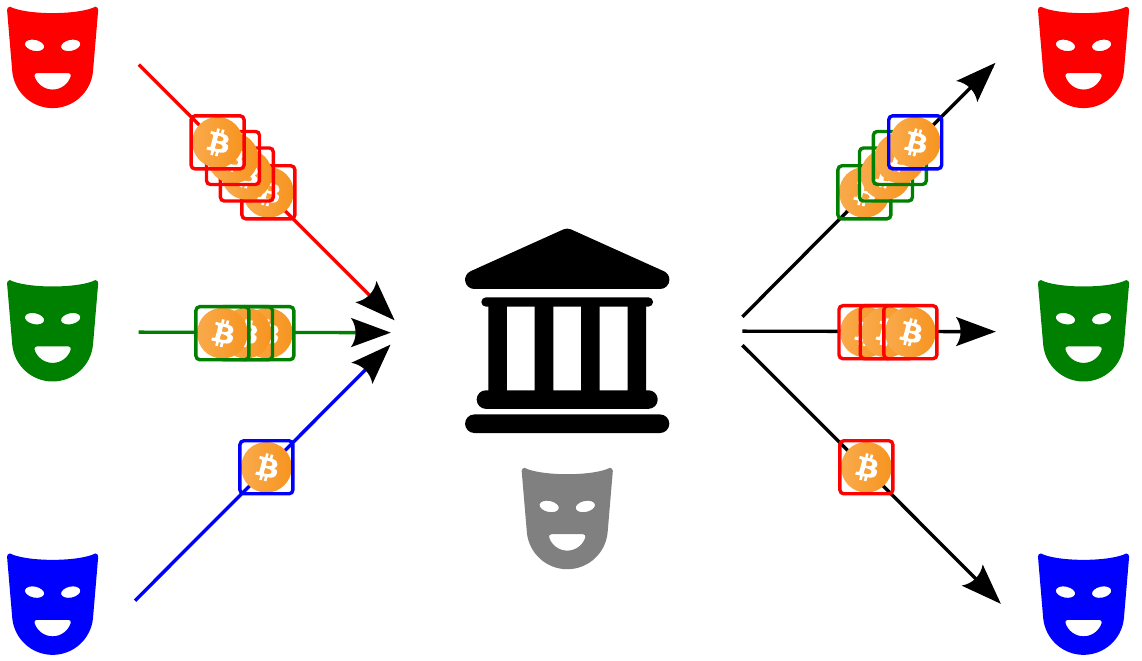
\includegraphics[width=1\linewidth]{img/mixing-service-scheme.png}
	\caption{Scheme of how a mixing service works}
	\label{fig:mixing-service-scheme}
\end{figure}






%%%%%%%%%%%%%%%%%%%%%%%%%%%
% *** SECOND SUB-SECTION ***
%%%%%%%%%%%%%%%%%%%%%%%%%%%
\subsection{Enhancing privacy through blind signatures}\label{sec:enh-sign} In
the following section is presented a mixing service scheme for enhancing Bitcoin
privacy through the use of blind signatures. The scheme has been proposed  by E.
Heilman, F. Baldimtsi and S. Goldberg \cite{heilman-blindly-signed-contracts},
is based on the scheme used in eCash \cite{Chaum1984} and, unlike other previous
schemes that are efficient but achieve limited security/anonymity or other which
provide strong anonymity but are slow and require large numbers of transactions,
it provides anonymity at reasonable speed using an untrusted third party (which
can, therefore, be malicious).

\subsubsection{High-level overview of the scheme}
\paragraph{Scenario}
The scenario is the following: $A$, \emph{the payer}, wants to anonymously send
1 bitcoin to $B$, \emph{the  payee}. If $A$ performed a standard transaction
sending 1 BTC from $address_A$ (owned by $A$) to a fresh ephemeral address
$address_B$ (owned by $B$), there would be a record in the blockchain linking
the two addresses. Even if $A$ and $B$ always create a fresh address for each
payment they receive, the links between addresses can be used to de-anonymize
users when they for example have a transaction with a third party which learns
their identify (e.g. their email address). The basic idea is to used a third
party $I$ that breaks the link between $A$ and $B$ addresses: $A$ sends coins to
$I$ and $I$ sends different coins for the same value to $B$, acting thus as a
mixing service. If other users use $I$ and enough transactions pass through it,
it becomes difficult for an attacker to link $A$ and $B$.

\emph{The main problem is that $I$ knows everything about the transactions between
$A$ and $B$}.

\paragraph{eCash scheme}
A possible solution to this issue is the scheme used in eCash for preventing $I$
from knowing who $A$ wants to pay. This scheme is shown in figure
\ref{fig:eCash-scheme} and relies on blind signatures. $A$ chooses a random
serial number $sn$, blinds it to $\overline{sn}$ and asks $I$ to compute a blind
signature $\overline\sigma$ on $\overline{sn}$, which sends back to $A$. $A$
unblinds these values to obtain $V = (sn, \sigma)$ and then pays $B$ using the
voucher $V$. Finally, $B$ redeems $V$ with $I$ to obtain the bitcoin. With this
scheme $I$ does not know who $A$ wants to pay it cannot read the blinded serial
number $\overline{sn}$ that it signs and it cannot link a message/signature
$(sn, \sigma)$ pair to its blinded value $(\overline{sn}, \overline\sigma)$.
Blindness, therefore, ensures that $I$ cannot link a voucher it redeems with a
voucher it issues. Blind signatures are also unforgeable, which ensures that a
malicious user cannot issue a valid voucher to itself.
\begin{figure}[!htb]
	\centering
	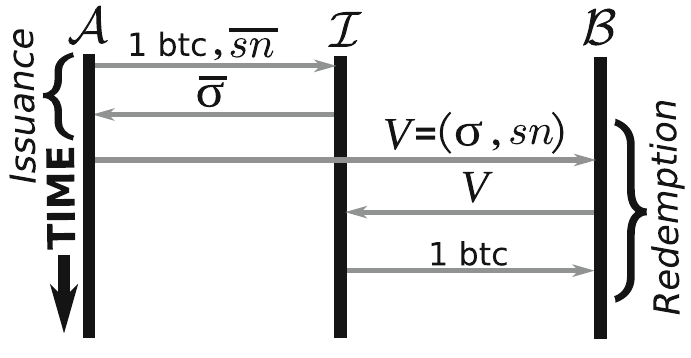
\includegraphics[width=0.6\linewidth]{img/eCash-scheme.png}
	\caption{eCash protocol scheme}
	\label{fig:eCash-scheme}
\end{figure}

\paragraph{Heilman scheme} The main problem with the eCash approach is that $I$
has to be honest: if $I$ is malicious it could refuse to issue a voucher to $A$
after receiving its bitcoin and thus the scheme fails. To solve this, the scheme
proposed in \cite{heilman-blindly-signed-contracts} uses Bitcoin
\emph{transaction contracts} for achieving blockchain-enforced \emph{fair
exchange}. An high-level view of the scheme is shown in figure
\ref{fig:heilman-scheme}. The scheme consists of four blockchain transactions
that are confirmed in three blocks on the blockchain and the key idea is that
$A$ transfers a bitcoin to $I$ if and only if it receives a valid voucher $V$ in
return. The four transactions implement two fair exchanges:
\begin{itemize}
  \item $V\rightarrow BTC$, which consists of the transactions (1) $T_{offer(V\rightarrow
  BTC)}$ and (2) $T_{fulfill(V\rightarrow BTC)}$ and it ensures that a malicious $I$
  cannot redeem $B$’s voucher without providing $B$ with a bitcoin in return.
  The exchange stands in for the interaction between $B$ and $I$.
  Transaction (1) offers a fair exchange of one bitcoin (from $I$) for
  one voucher (from $B$), while transaction (2) is created by $B$ to meet
  the offer by $I$.
  \item $BTC\rightarrow V$, which consists of the two transactions (1) $T_{offer(BTC\rightarrow
  V)}$ and (2) $T_{fulfill(BTC\rightarrow V)}$ and it ensures that a malicious $I$
  cannot take a bitcoin from $A$ without providing it with a voucher $V$.
\end{itemize}


\begin{figure}[!htb]
	\centering
	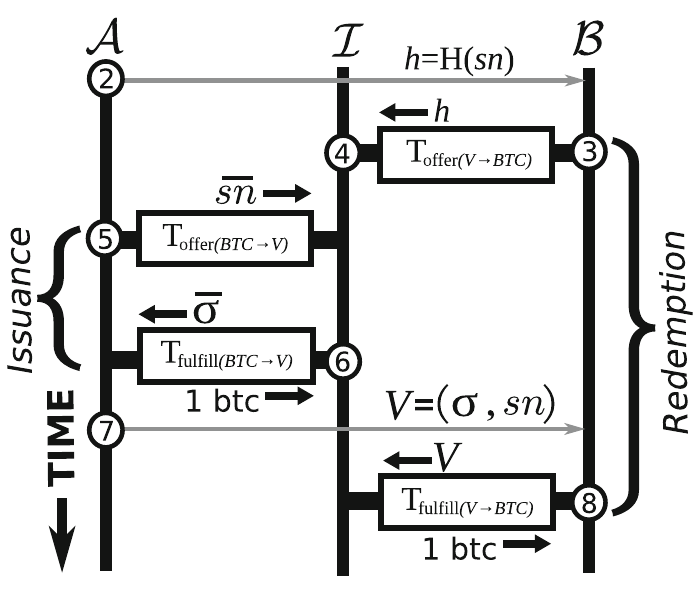
\includegraphics[width=0.6\linewidth]{img/heilman-scheme.png}
	\caption{High-level view of the scheme proposed in \cite{heilman-blindly-signed-contracts}}
	\label{fig:heilman-scheme}
\end{figure}

\subsubsection{Fair exchange implementation} In the following section, it will be
explained how the transaction contracts $T_{offer(BTC\rightarrow V)}$ and (2)
$T_{fulfill(BTC\rightarrow V)}$ implement the fair exchange $BTC\rightarrow V$
used in our protocol scheme shown in figure \ref{fig:heilman-scheme}. The
implementation for the exchange $V\rightarrow BTC$ is analogous.

As already mentioned, the fair exchanges are achieved using transaction
contracts. A transaction contract can be implemented using \emph{Script}, a
simple programming language provided by Bitcoin which, as discussed in chapter
\ref{sec:scripts}, allows to associate each transaction with a script which
defines the rules for spending the transaction outputs, namely how the next
person wanting to spend the bitcoins being transferred can gain access to them.

In this case, the CHECKLOCKTIMEVERIFY feature of Script is used in order to
timelock a transaction, so that funds can be reclaimed if a contract has not
been spent within a given time window $tw$. For implementing the $BTC\rightarrow
V$ fair exchange, $A$ generates the transaction contract
$T_{offer(BTC\rightarrow V)}$ which says the following:

``\emph{$A$ offers bitcoins to $I$ under the condition that $I$ must compute a
valid blind signature on the blinded serial number $\overline{sn}$ (provided by $A$)
within time window $tw$. If this condition is not satisfied, the
bitcoin reverts to $A$.}''

The output of this transaction therefore can be spent in a future transaction $T_f$
only if one of the following conditions is met:
\begin{enumerate}
  \item $T_f$ is signed by $I$ and contains a valid blind signature $\overline\sigma$ on $\overline{sn}$
  \item $T_f$ is signed by $A$ and the time window $tw$ has expired.
\end{enumerate}
For fulfilling the contract and acquiring the bitcoins of the transaction $I$
has therefore to satisfy the condition $2$, which means that $I$ has to post a
transaction $T_{fulfill(BTC\rightarrow V)}$ that contains a valid blind
signature $\overline\sigma$ on $\overline{sn}$. If $I$ does not fulfill the
contract within the time window $tw$, then the condition $2$ is met when $A$
signs and posts a transaction $T_f$ that returns back the offered bitcoins.

\subsubsection{Blind signature scheme} The scheme used for the blind signature
is the Boldyreva’s scheme \cite{boldyreva2003threshold}, which requires two
rounds of interaction. Since the elliptic curve defined by the standard
Secp256k1 used by Bitcoin doesn't support the bilinear pairings required for the
adopted signature scheme, for using the scheme it is necessary to slightly
modify the Bicoin protocol in order to adopt a different elliptic curve.

Let $\mathbb{G}$ be a cyclic additive group of order $p$ (with $p$ prime) in
which the Diffie-Hellman problem is hard and $\mathbb{G'}$ a cyclic
multiplicative group of prime order $q$. Let $e\colon
\mathbb{G}\times\mathbb{G}\to\mathbb{G'}$ be the bilinear pairing, $g$ be a
generator of the group $\mathbb{G}$ and $H$ be a hash function mapping arbitrary
strings to elements of $\mathbb{G}\setminus \{1\}$. The public parameters are
$(p, g, H)$ while the signer public/private key pair is $(sk , pk = g^{sk})$.
The signature scheme works as follow:
\begin{itemize}
  \item To blind $sn$, user $A$ picks random $r\in \mathbb{Z}^{*}_p$ and sets
  $\overline{sn}=H(sn)g^r$.
  \item To sign $\overline{sn}$, signer $I$ computes $\sigma = \overline{sn}^{sk}$.
  \item To unblind the blind signature $\overline{\sigma}$, user $A$ computes
  $\sigma = \overline{\sigma} {pk}^{\-- r}$.
  \item To verify the signature $\sigma$ on $sn$, anyone holding $pk$ checks
  that the bilinear pairing $e(pk,H(sn))$ is equal to $e(g,\sigma)$.
  For verifying the blinded signature $\overline\sigma$ on the blinded
  $\overline{sn}$, anyone holding $pk$ checks if $e(pk,\overline m)= e(g,\overline\sigma)$.
\end{itemize}


\subsubsection{Anonymity considerations} While in the eCash protocol of figure
\ref{fig:eCash-scheme} the anonymity level of users depends on the total number
of payments using $I$, in the scheme proposed by Heilman shown in figure \ref{fig:heilman-scheme} the anonymity level
depends on the number of payment through $I$ in a given epoch. The protocol, in
fact, runs in epochs and provides set-anonymity within each epoch. An epoch is the
three-blocks window in which the four transactions required by the protocol are
confirmed and stored, as shown in figure \ref{fig:epochs}.
\begin{figure}[!htb]
	\centering
	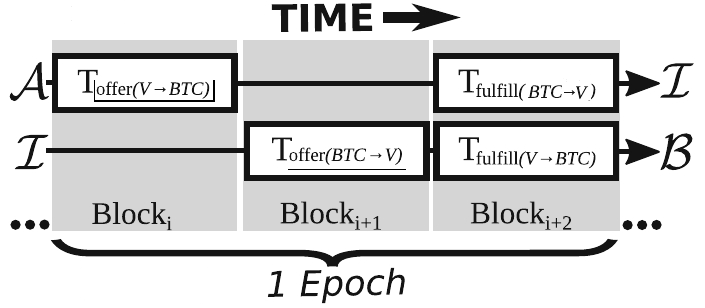
\includegraphics[width=0.6\linewidth]{img/epochs.png}
	\caption{}
	\label{fig:epochs}
\end{figure}

The anonymity considerations about the proposed scheme are based on the following
assumptions:
\begin{itemize}
  \item all the users coordinate on epoch so that the transactions arrangement
  shown in figure \ref{fig:epochs} is respected (e.g. they choose the starting
  block so that its height\footnote{height=distance from the genesis block}
  is multiple of three)
  \item the payer $A$ and the payee $B$ trust each other. If $A$ or $B$ were malicious
  they could easily conspire with $I$ revealing the other part identity: for example
  $A$ could comunicate $I$ the serial number of the received voucher so that when
  $I$ can identify $B$ when he redeems that voucher
  \item payees B always receive payments in a fresh ephemeral address $address_B$
  \item payers only make one anonymous payment per epoch. Similarly, payees only
  accept one payment per epoch.
\end{itemize}

\paragraph{Epoch set-anonymity} As consequence of assumptions (2) and (3), in
every epoch there are exactly $n$ addresses making payments (playing the role of
payer $A$) and $n$ receiving addresses (playing the role of $B$). Anyone looking
at the blockchain can therefore see the participating addresses of payers and
payees, but the probability of successfully linking any chosen payer $A$ to a
payee $B$ should not be more than $1/n$, namely an attacker observing the
blockchain can do no better than randomly guessing who paid whom during an epoch.

\paragraph{Transparency of anonymity} Users learn the size of their anonymity
set (number of participants in their epoch) only after a transaction completes
by looking at the blockchain. If particular $B$ feels his anonymity set is too
small in one epoch, he can increase the size of it by using the scheme as  a
mixing service and making a new transaction to another address owned by him. For
example:  $address_B$ gets paid in an epoch with $n = 4$. $B$ can create a fresh
ephemeral address $address'_B$ and have $address_B$ pay $address'_B$ in a
subsequent epoch. If the subsequent epoch has a $n = 100$, then B increases the
size of his anonymity set.

\paragraph{Intersection attack} As pointed out by the autors in
\cite{heilman-blindly-signed-contracts}, there's the possibility for an attacker
(or anyone looking at the blockchain) to attempt an intersection attack that
de-anonymaze users across different epochs by using frequencial analysis.


  \printbibliography

\end{document}
